\documentclass[10pt,a4paper]{beamer}
\usepackage[utf8]{inputenc}
%\usepackage[german]{babel}
\usepackage[T1]{fontenc}
\usepackage{amsmath}
\usepackage{amsfonts}
\usepackage{amssymb}
\usepackage{ulem}
\usepackage{tikz}
\usetikzlibrary{decorations.pathmorphing,calc}
\usepackage{dirtytalk}
\author{Daniel Kirchner}
\title{Applying Computational Methods\\to a Foundational Metaphyiscal Theory}
%\date{9th of May, 2022}
\date{June 1, 2022}
\institute{Workshop on Computational Metaphysics and Intensionality\\University of Bamberg}

%\setbeamertemplate{frame footer}{Disputation}


%\setbeamertemplate{footline}[text line]{\hfill Disputation Daniel Kirchner, Fachbereich Mathematik und Informatik der Freien Universit\"at Berlin}
\setbeamertemplate{footline}[frame number]{}
\setbeamertemplate{navigation symbols}{}
\begin{document}

\begin{frame}
\frametitle{Extensional, non-modal Aczel model of second-order AOT}
\tikzset{font=\fontsize{8pt}{10pt}\selectfont}
\begin{columns}
\begin{column}{0.7\textwidth}
\begin{figure}[H]
\centering
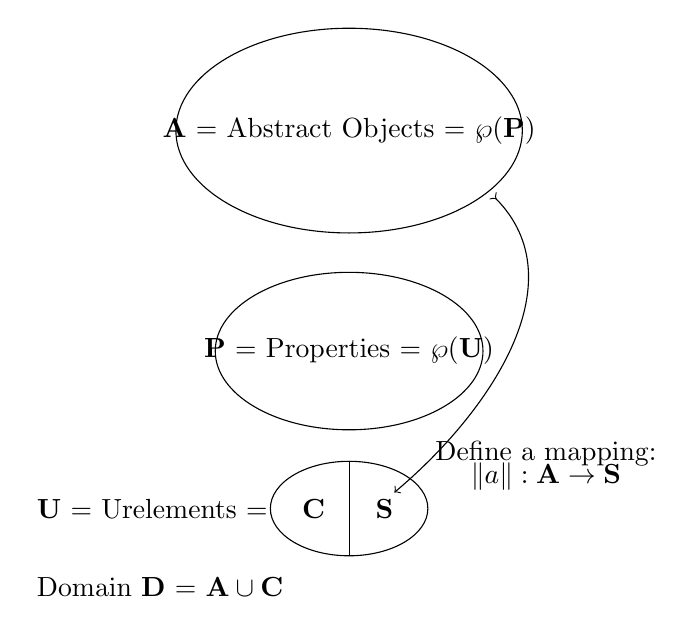
\begin{tikzpicture}

% Domains
 \node at (-2.4,-1) {Domain \textbf{D} = $\mathbf{A} \cup \mathbf{C}$};

% \node at (-.8,-1.5) {Define for $\mathitbf{x}\in \textbf{D}$, $|\mathitbf{x}| = 
%   \left\{\begin{array}{ll}
%      \hspace*{-.05in}\mathitbf{x}, \textrm{when}\  \mathitbf{x}\in \mathbf{C}\\
%      \hspace*{-.05in}\|\mathitbf{x}\|, \textrm{when}\  \mathitbf{x}\in 
% \mathbf{A}
%    \end{array}
%   \right.$};

% U
 \draw (0,0) ellipse (1 and .6);
 \draw (0,.6) -- (0,-.6);
 \node at (-2.5,0) {\textbf{U} = Urelements =};
 \node at (2.5,.7) {Define a mapping:};
 \node at (2.5,.4) {$\|a\| : \textbf{A} \to \textbf{S}$};
 \node at ($(-.45,.8)+(-90:1 and .6) + (0,-.2)$) {\textbf{C}};
 \node at ($(.45,.8)+(-90:1 and .6) + (0,-.2)$) {\textbf{S}};
 \node (S) at ($(.45,.9)+(-90:1 and .6) + (0,-.2)$) {};

% P
 \draw (0,2) ellipse (1.7 and 1);
 \node at (0,2) {\textbf{P} = Properties = $\wp (\mathbf{U})$};

% A
 \draw (0,4.8) ellipse (2.2 and 1.3);
 \node at (0,4.8) {\textbf{A} = Abstract Objects = $\wp (\mathbf{P})$};
 \node (A) at (1.7,4.1) {};


% Arrows
 \draw [>->] (A) to[out=-45, in=40] (S);

\end{tikzpicture}
\end{figure}
\end{column}
\begin{column}{0.3\textwidth}
\begin{equation*}
  |x| =
  \begin{cases}
    x\mbox{, if } x \in C \\
    ||x||\mbox{, if } x \in A
  \end{cases}
\end{equation*}

$Fx$ is true, if $|x| \in F$\\
\vspace{1em}
$xF$ is true,\\if $x \in A$ and $F \in x$\\
\end{column}
\end{columns}
\end{frame}


\end{document}
